\section{Observations}
\begin{enumerate}[I.]
\item Firstly, we observe that walls are oriented away from the path they face as can be seen in Figure~\ref{PathNormal}. The walls connect to neighbours, and non-corner walls face into the normal of the direction of the path. Because of the walls' asymmetry there are two different ways to face the path, one ''clamped'' towards and one away. Consistently clamping in the same direction establishes the visual conditions of the walls. Thus the problem reduces to finding normal of the wall square's adjacent path, and consistently clamping away in relation to it.
\begin{figure}[H]
	\centering
	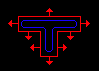
\includegraphics[width=0.4\linewidth]{Image-6.png}
	\caption {Arrows show the normal to the path that surrounds the boundary formed by the walls.\autocite{myself}} \label{PathNormal}
\end{figure}

\item To find the normal to the direction of the path around the walls, we must first know the direction of the path adjacent to each wall square. Since the walls, forming the boundary, define the path that surrounds, as they serve as an outline of it, we must find the closed path which the walls themselves form.\label{ClosedPathObservation} Instead of using the path adjacent to the walls as a rule of determining the tiles' orientation, we will use the tiles themselves in relation to each other, to trace their boundary thus finding the normal of that outline and solving the problem.

\item Since the walls each represent a single square in a rectangular 2D grid of integer coordinates, we can map them onto a square lattice graph as can be seen in Subfigure~\ref{BoundaryLattice}.\label{SquareLatticeObservation}

\begin{figure}[H]
	\begin{subfigure}[b]{0.5\textwidth}
		\centering
		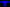
\includegraphics[width=0.7\linewidth]{Image-7.png}
		\caption {Pixel representation of a boundary formed by walls.\autocite{myself}}\label{PixelBoundary}
	\end{subfigure}
	\begin{subfigure}[b]{0.5\textwidth}
		\centering
		\tikz[every node/.style={draw,circle}] \graph [no placement] {
			a [x=0,y=3] -- b [x=1,y=3] -- c[x=2,y=3] -- d[x=3,y=3] -- e[x=4,y=3] -- f[x=5,y=3] -- g[x=5,y=2] -- h[x=4,y=2] -- i[x=3,y=2] -- j[x=3,y=1] -- k[x=3,y=0] -- l[x=2,y=0] -- m[x=2,y=1] -- n[x=2,y=2] -- o[x=1,y=2] -- p[x=0,y=2] -- a;
			b -- o;
			c -- n;
			d -- i;
			e -- h;
			n -- i;
			m -- j;
		};
		\caption {Corresponding lattice graph of the wall configuration in~\ref{PixelBoundary}\autocite{myself}}\label{BoundaryLattice}
	\end{subfigure}
	\caption {Two representations of graph boundaries.}
\end{figure}

\item We can find a Hamiltonian cycle of the square lattice of the walls of a Pacman level to find the path defining its boundary to solve the problem, accounting for observations~\ref{ClosedPathObservation} and~\ref{SquareLatticeObservation}.

\begin{figure}[H]
	\centering
	\tikz[every node/.style={draw,circle}] \graph [no placement] {
		a [x=0,y=3] -> b [x=1,y=3] -> c[x=2,y=3] -> d[x=3,y=3] -> e[x=4,y=3] -> f[x=5,y=3] -> g[x=5,y=2] -> h[x=4,y=2] -> i[x=3,y=2] -> j[x=3,y=1] -> k[x=3,y=0] -> l[x=2,y=0] -> m[x=2,y=1] -> n[x=2,y=2] -> o[x=1,y=2] -> p[x=0,y=2] -> a;
		b -- o;
		c -- n;
		d -- i;
		e -- h;
		n -- i;
		m -- j;
		{[edges={red,line width=2pt}] a->b->c->d->e->f->g->h->i->j->k->l->m->n->o->p->a}
	};
	\caption {Desired Hamiltonian cycle for lattice graph in Figure~\ref{BoundaryLattice}}\label{HamiltonianBoundaryLattice}
\end{figure}

\end{enumerate}